\chapter{Experimental setup}
\section{Selected datasets}
\label{sec:selected_datasets}
A summary of the list of datasets used for the empirical study, performance estimation and ranking of error detection strategies can be found below (\autoref{tab:dataset-error-types}). The datasets were taken from published data from the following papers: 
\begin{itemize}
    \item ED2 by \cite{Neutatz2019-aw}
    \item Raha by \cite{Mahdavi2019-zf}
    \item REDS by \cite{Mahdavi2019-pk}
    \item CleanML by \cite{Li2019-ve}
\end{itemize}

\autoref{tab:dataset-error-types} shows each of the datasets and the common error types that occur in these datasets. Statistics about the used datasets can be found in \autoref{tab:dataset_statistics}. Below, a general description of all datasets will be presented and the source of the dataset will be mentioned.

\begin{table}[]
\begin{adjustbox}{width=\textwidth,center}
\begin{tabular}{|l|c|c|c|c|c|}
\hline
\textbf{Dataset name} & \textbf{Pattern violations} & \textbf{Rule violations} & \textbf{Outliers} & \textbf{Duplicates} & \textbf{Other error types} \\ \hline
\textit{Airbnb}       &                   & \checkmark                                    & \checkmark                             & \checkmark          &                                                 \\ \hline
\textit{Beers}        & \checkmark                                       & \checkmark                                    &                                        &                     &                                                 \\ \hline
\textit{EEG}          &                                                  &                                               & \checkmark                             &                     & \checkmark                                      \\ \hline
\textit{Flights}      & \checkmark                                       & \checkmark                                    &                                        &                     &                                                 \\ \hline
\textit{Hospital}     & \checkmark                                       &                                               &                                        &                     &                                                 \\ \hline
\textit{Marketing} & & \checkmark & & & \checkmark \\ \hline
\textit{Movie}        &                                                  & \checkmark                                    &                                        &  \checkmark                   &                                                 \\ \hline
\textit{Movies}       & \checkmark                                       & \checkmark                                    &                                        &                     & \checkmark                                      \\ \hline
\textit{Rayyan}       & \checkmark                                       & \checkmark                                    &                                        &                     &                                                 \\ \hline
\textit{Restaurant}   & \checkmark                                       & \checkmark                                    &                                        &                     &                                                 \\ \hline
\textit{Restaurants}  & \checkmark                                       &                                               &                                        &                     &                                                 \\ \hline
\textit{Toy}          &                                                  & \checkmark                                    &                                        &                     & \checkmark                                      \\ \hline
\textit{University}   &                                                  & \checkmark                                    &                                        &                     &                                                 \\ \hline
\textit{Uscensus}     &                                                  & \checkmark                                    &                                        &                     & \checkmark                                      \\ \hline
\end{tabular}
\end{adjustbox}
\caption{Datasets used and the common error types present in these datasets}
\label{tab:dataset-error-types}
\end{table}

\paragraph{AirBnb}
This dataset contains 42,492 records on hotels in the top 10 tourist destinations and major US metropolitan areas scraped from Airbnb.com. Each record has 40 attributes including the number of bedrooms, price, location, etc. Demographic and economic attributes were scraped from city-data.com. The classification task is to determine whether the rating of each hotel is 5 or not.
\\(Source: CleanML)

\paragraph{Beers} 
This dataset contains a list of different beers. The attributes are numeric ID's, foreign keys, names, City, state abbreviation, includes amount of ounces \& percentage alcohol.
\\(Source: ED2, REDS, Raha)

\paragraph{EEG}
This is a dataset of 14,980 EEG recordings. Each record has 14 EEG attributes. One of the attributes is a classification task is to predict whether the eye-state is closed or open. In the dirty version of this dataset, some of these predictions are wrong.
\\(Source: CleanML)

\paragraph{Flights}
This dataset contains a flight schedule. Attributes are id, source of data, flight number alphanumeric with dashes, scheduled and actual departure and arrival times in XX:XX a.m. format.
\\(Source: ED2, REDS, Raha)

\paragraph{Hospital}
This source contains a list of hospital experiments. Attributes include ID, hospital names, addresses, measurement types, measurement named, experiment scores and other statistics about the hospital and experiments.
\\(Source: REDS, Raha)

\paragraph{Marketing}
This dataset consists of 8,993 records about household income from a survey. Each record has 14 demographic attributes including sex, education, etc. Another attribute is a classification task is to predict if the annual household income is less than \$25,000.
\\(Source: CleanML)

\paragraph{Movies}
This test set is a collection of popular movies. Attributes of this source are:
Id, Name, Year, Release Date, Director, Creator, Actors, Cast, Language, Country, Duration, RatingValue, RatingCount, ReviewCount, Genre, Filming Locations, Description
\\(Source: ED2, REDS, Raha)

\paragraph{Movie}
Same as movies, but less and different columns
\\(Source: CleanML)

\paragraph{Rayyan}
This dataset contains a set of published articles. The attributes include the title, which journal it was published in, the date, pagination and other information important for citing the articles.
\\(Source: REDS, Raha)

\paragraph{Restaurants}
This source is a list of restaurants. Attributes contain the name, address, phone number, website and other attributes that our commonly found on restaurant review websites (like rating value and price range).
\\(Source: ED2)

\paragraph{Restaurant}
Same idea as "Restaurants", but less columns.
\\(Source: CleanML)

\paragraph{Toy}
Dummy set for testing purposes \& testing for generalizability
\\(Source: REDS, Raha)

\paragraph{University}
This dataset contains 286 records about universities. Each record has 17 attributes including state, university name, SAT scores, etc. It contains a column with a classification task is to predict whether the expenses are greater than 7,000 for each university. This dataset contains inconsistent representations for states and locations.
\\(Source: CleanML)

\paragraph{Uscensus}
This dataset contains 32,561 US Census records for adults. Each record has 14 attributes including age, education, sex, etc. It also contains an attribute with a classification goal of predicting whether the adult earns more than \$50,000. 
\\(Source: CleanML)


\begin{table}
\begin{tabular}{llrrrr}
\toprule
     Dataset & Data quality &   Rows &  Columns &  Number of errors &  Total cells \\
\midrule
      airbnb &       85.4 \% &  18406 &       40 &            107625 &       736240 \\
       beers &       83.5 \% &   2410 &       11 &              4362 &        26510 \\
         eeg &       97.6 \% &  14980 &       15 &              5496 &       224700 \\
     flights &       70.4 \% &   2376 &        7 &              4920 &        16632 \\
    hospital &       97.5 \% &   1000 &       20 &               509 &        20000 \\
   marketing &       78.7 \% &   8993 &       14 &             26815 &       125902 \\
       movie &       63.3 \% &   6531 &        8 &             19174 &        52248 \\
      movies &       98.8 \% &   7390 &       17 &              1501 &       125630 \\
      rayyan &       91.4 \% &   1000 &       11 &               948 &        11000 \\
  restaurant &       99.5 \% &  12007 &       11 &               635 &       132077 \\
 restaurants &       99.9 \% &  28787 &       16 &               565 &       460592 \\
         toy &       77.8 \% &      6 &        3 &                 4 &           18 \\
  university &       97.4 \% &    210 &       18 &               100 &         3780 \\
    uscensus &       99.1 \% &  32561 &       15 &              4262 &       488415 \\
\bottomrule
\end{tabular}
\caption{Dataset statistics}
\label{tab:dataset_statistics}
\end{table}

\section{Metrics}
\label{sec:metrics}
To measure the performance of tools on test datasets, metrics of two types can be used. Cell-based and row-based metrics. The difference lies in what is taken as an entity while calculating scores.

\subsubsection{Cell-based metrics}
Cell-based metrics, are metrics that identify each cell in a dataset as a separate entity in the test set. Each cell will be counted as 1 positive or negative. 

\subsubsection{Row-based metrics}
Row-based metrics, are metrics that identify each row in a dataset as a separate entity in the test set. A row could contain multiple errors, but only the whole row is counted as 1 positive or negative.

\subsubsection{Scores}
In the case of error detection, instances are either erroneous (positive) or clean (negative). Because the ground truth of the datasets in \autoref{subsec:datasets} is known, the performance metrics can be calculated directly after the execution of a tool. 
The following performance scores will be kept after experiments and estimated in the later stages of the research:
\begin{itemize}
    \item Precision ($= \frac{\text{true positives}}{\text{true positives} + \text{false positives}}$)
    \item Recall ($= \frac{\text{true positives}}{\text{true positives} + \text{false negatives}}$)
    \item F1-score ($= 2 \cdot \frac{\text{precision} \cdot \text{recall}}{\text{precision} + \text{recall}}$)
\end{itemize}

\subsubsection{Examples}
To provide visual aid for the different metrics proposed, examples are shown in \autoref{fig:error_row_wise}. In the figure, the real errors (difference between dirty dataset and the ground truth) are labeled cell-wise by underling and displaying in bold. The "detected" errors by the fictional error detection strategies are shown with a red background. In contrast to the cell-wise detection, the erroneous rows are marked by the black arrows to the left. The "detected" faulty rows are marked by the red arrows on the right.

\begin{figure}[h]
\centering
    \begin{subfigure}{0.9\textwidth}
        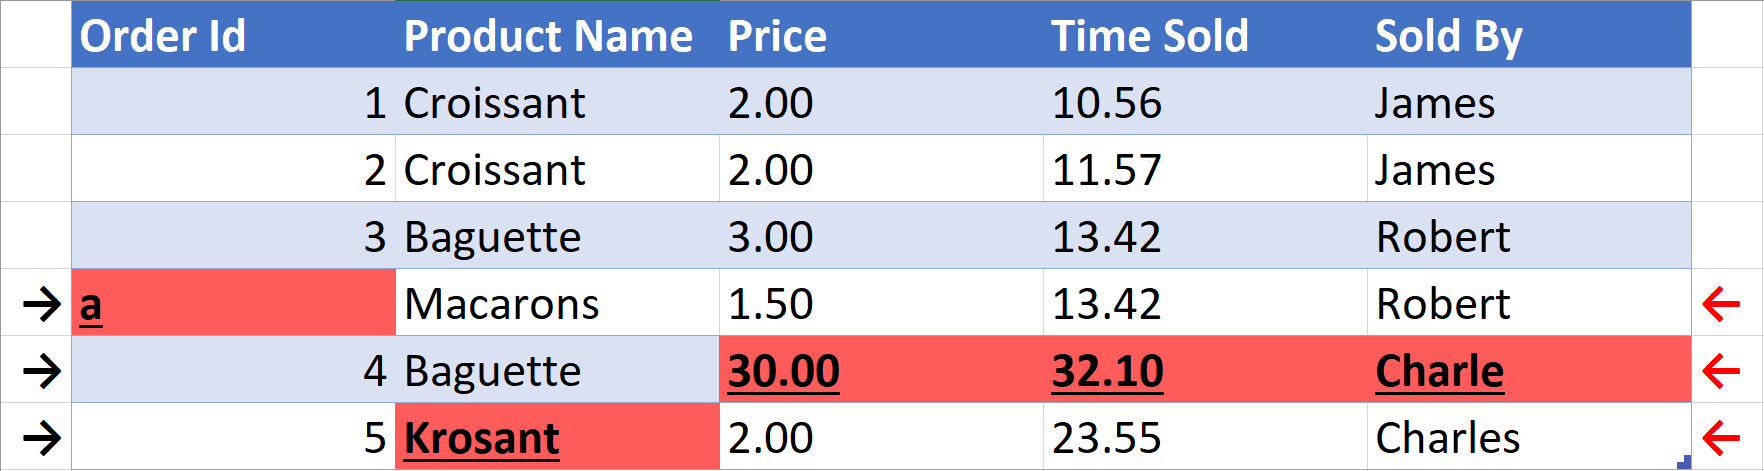
\includegraphics[width=\linewidth]{thesis/Figures/Method/Errors_dataset_F1_row.png}
        \caption{}
        \label{subfig:errors_row}
    \end{subfigure}
    \begin{subfigure}{0.9\textwidth}
        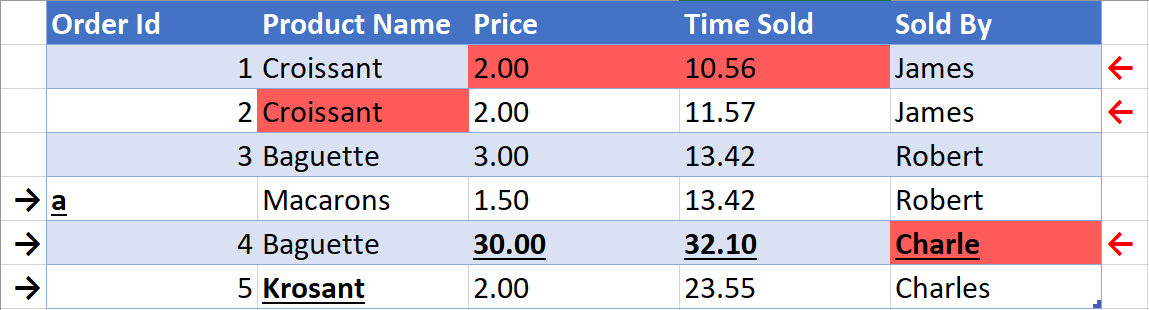
\includegraphics[width=\linewidth]{thesis/Figures/Method/Errors_dataset_Worse_F1_row.png}
        \caption{}
        \label{subfig:errors_row_worse}
    \end{subfigure}
    \caption{Two examples of error detection. Real errors are underlined and bold. Example outputs by error detection methods are marked in red.}
    \label{fig:error_row_wise}
\end{figure}

~\\\textbf{Cell-wise scores} in the examples are as follows. 
\\For \autoref{subfig:errors_row}, there is a total of 5 real error cells. The detection algorithm marks all 5 errors correctly. So $precision = \frac{5}{5} = 1$, $recall = \frac{5}{5} = 1$ and $F1 = 2 \times \frac{1 \times 1}{1 + 1} = 1$. 
\\For \autoref{subfig:errors_row_worse}, there are also the same 5 real error cells. The detection algorithm marks only 1 error correctly and 3 more incorrectly. So $precision = \frac{1}{4} = 0.25$, $recall = \frac{1}{5} = 0.2$ and $F1 = 2 \times \frac{0.25 \times 0.2}{0.25 + 0.2} = 0.22$. 

~\\\textbf{Row-wise scores} for the two examples are different than the cell-wise performance scores.
\\For \autoref{subfig:errors_row}, there is a total of 3 real error rows. The detection algorithm marks all 3 rows correctly. So $precision = \frac{3}{3} = 1$, $recall = \frac{3}{3} = 1$ and $F1 = 2 \times \frac{1 \times 1}{1 + 1} = 1$. 
\\For \autoref{subfig:errors_row_worse}, there are also the same 3 real error rows. The detection algorithm marks only 1 row correctly and 2 more incorrectly. So $precision = \frac{1}{3} = 0.33$, $recall = \frac{1}{3} = 0.2$ and $F1 = 2 \times \frac{0.33 \times 0.33}{0.33 + 0.33} = 0.33$. 

\begin{table}[h]
\centering
\begin{tabular}{l|lll}
\textbf{}    & \textbf{Precision} & \textbf{Recall} & \textbf{F1} \\ \hline
\textbf{(A)} & 1 / 1              & 1 / 1           & 1 / 1       \\
\textbf{(B)} & 0.25 / 0.33        & 0.2 / 0.33      & 0.22 / 0.33
\end{tabular}
\caption{Cell-wise / Row-wise performance score differences for the two examples in \autoref{fig:error_row_wise}}
\label{tab:cell_vs_row_scores}
\end{table}

~\\For this research, \textbf{cell-wise scores} will be used to measure the performance of error detection strategies. The goal of error detection in this thesis is to holistically find all different types of errors. Unlike for example duplicate rows, most other errors are defined only for single cells. To also include duplicate rows in the scoring, the complete row is marked as erroneous. The error detection algorithms will be scored accordingly.

\section{Error detection tool configurations}
After generating configurations with the settings shown in \autoref{sec:empiricalstudy}, the number of strategies per tool are shown in \autoref{tab:number_configs_tool}. However, not all strategies will be able to produce results within the timeouts.

\begin{table}[H]
\centering
\begin{tabular}{lr}
\toprule
Tool &  Number of strategies \\
\midrule
dBoost            &                  72 \\
Raha              &                  37 \\
ForbiddenItemSets &                   7 \\
ActiveClean       &                   7 \\
KATARA            &                   4 \\
FAHES             &                   4 \\
\bottomrule
\end{tabular}
\caption{Number of configurations per tool}
\label{tab:number_configs_tool}
\end{table}


\section{Computer specification}
Experiments were run on a computer with an Intel Core i7 8750H processor using 16 GB of RAM, running Ubuntu 18.04 as Windows Subsystem for Linux 2. % running at 2.20 GHz base, 4.1 GHz max 
The max runtime for a single experiment was limited at 1800 seconds (half hour). A timeout error would occur after that and the experiment would be canceled. 